\documentclass{standalone}
\usepackage{tikz}
\usetikzlibrary{patterns, positioning}

\begin{document}
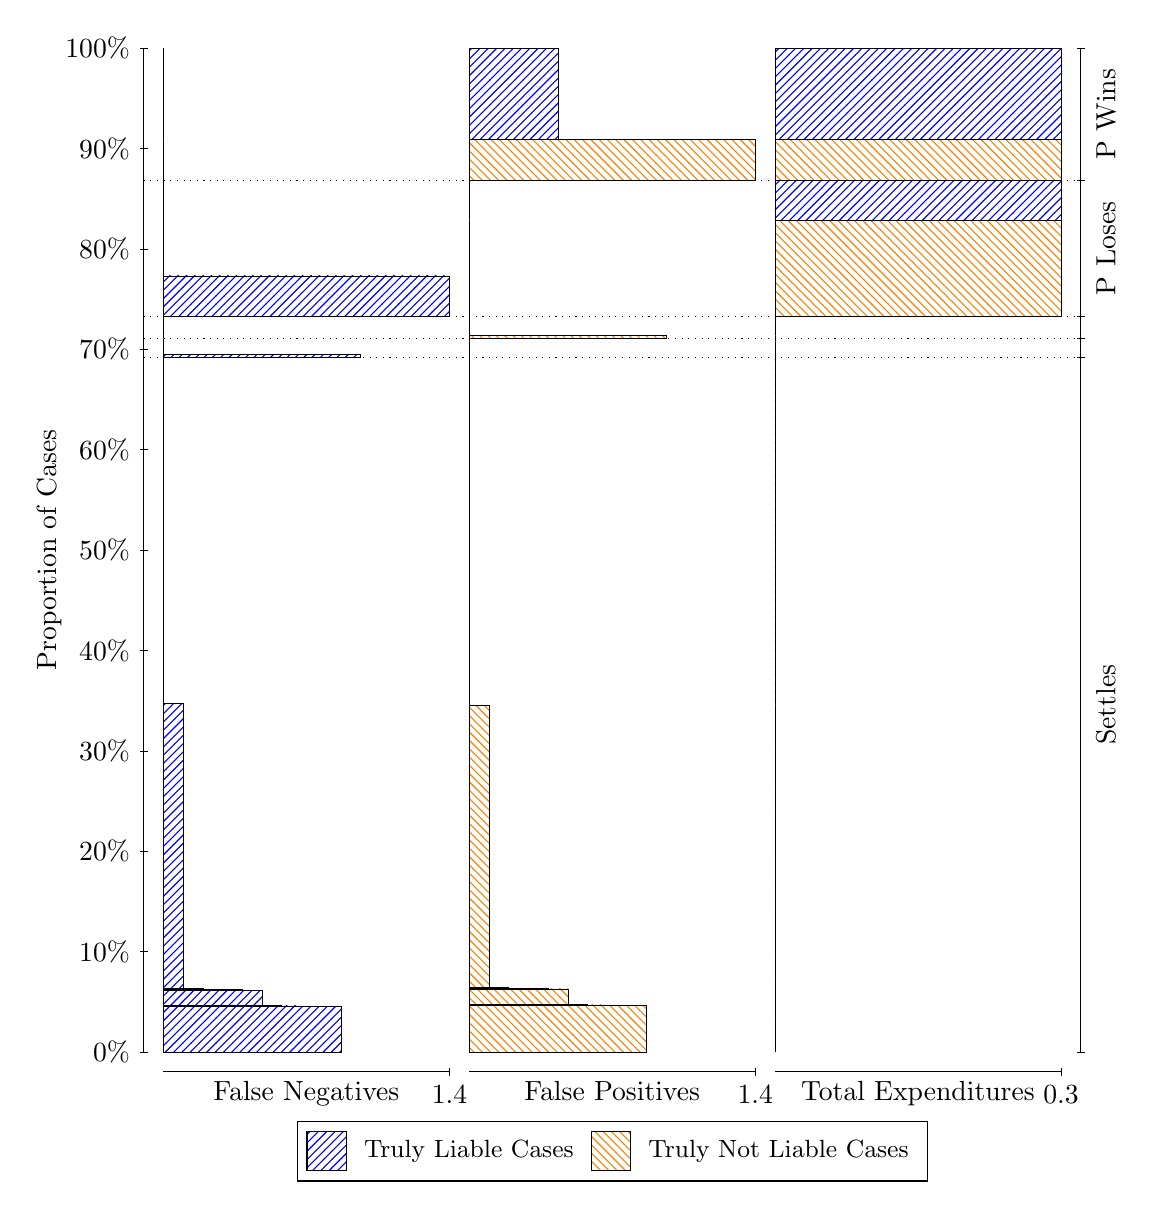
\begin{tikzpicture}
\draw[black, very thin] (1.5,1.75) -- (1.5,14.5);
\node[rotate=90, anchor=center] at (0.3, 8.125) {Proportion of Cases};
\draw[black, very thin] (1.45,1.75) -- (1.55,1.75);
\node[anchor=east] at (1.45, 1.75) {0\%};
\draw[black, very thin] (1.45,3.025) -- (1.55,3.025);
\node[anchor=east] at (1.45, 3.025) {10\%};
\draw[black, very thin] (1.45,4.3) -- (1.55,4.3);
\node[anchor=east] at (1.45, 4.3) {20\%};
\draw[black, very thin] (1.45,5.575) -- (1.55,5.575);
\node[anchor=east] at (1.45, 5.575) {30\%};
\draw[black, very thin] (1.45,6.85) -- (1.55,6.85);
\node[anchor=east] at (1.45, 6.85) {40\%};
\draw[black, very thin] (1.45,8.125) -- (1.55,8.125);
\node[anchor=east] at (1.45, 8.125) {50\%};
\draw[black, very thin] (1.45,9.4) -- (1.55,9.4);
\node[anchor=east] at (1.45, 9.4) {60\%};
\draw[black, very thin] (1.45,10.675) -- (1.55,10.675);
\node[anchor=east] at (1.45, 10.675) {70\%};
\draw[black, very thin] (1.45,11.95) -- (1.55,11.95);
\node[anchor=east] at (1.45, 11.95) {80\%};
\draw[black, very thin] (1.45,13.225) -- (1.55,13.225);
\node[anchor=east] at (1.45, 13.225) {90\%};
\draw[black, very thin] (1.45,14.5) -- (1.55,14.5);
\node[anchor=east] at (1.45, 14.5) {100\%};

\draw[black, very thin] (13.4,1.75) -- (13.4,14.5);
\draw[black, very thin] (13.35,1.75) -- (13.45,1.75);
\node[anchor=west] at (13.35, 1.75) {};
\draw[black, very thin] (13.35,10.57) -- (13.45,10.57);
\node[anchor=west] at (13.35, 10.57) {};
\draw[black, very thin] (13.35,10.81) -- (13.45,10.81);
\node[anchor=west] at (13.35, 10.81) {};
\draw[black, very thin] (13.35,11.09) -- (13.45,11.09);
\node[anchor=west] at (13.35, 11.09) {};
\draw[black, very thin] (13.35,12.821) -- (13.45,12.821);
\node[anchor=west] at (13.35, 12.821) {};
\draw[black, very thin] (13.35,14.5) -- (13.45,14.5);
\node[anchor=west] at (13.35, 14.5) {};

\draw[black, very thin, pattern color=blue, pattern=north east lines] (1.75,1.75) rectangle (4.0052,2.3257);
\draw[black, very thin, pattern color=blue, pattern=north east lines] (1.75,2.3257) rectangle (3.7546,2.3301);
\draw[black, very thin, pattern color=blue, pattern=north east lines] (1.75,2.3301) rectangle (3.504,2.3348);
\draw[black, very thin, pattern color=blue, pattern=north east lines] (1.75,2.3348) rectangle (3.2534,2.3395);
\draw[black, very thin, pattern color=blue, pattern=north east lines] (1.75,2.3395) rectangle (3.2534,2.3396);
\draw[black, very thin, pattern color=blue, pattern=north east lines] (1.75,2.3396) rectangle (3.0029,2.5365);
\draw[black, very thin, pattern color=blue, pattern=north east lines] (1.75,2.5365) rectangle (2.7523,2.5421);
\draw[black, very thin, pattern color=blue, pattern=north east lines] (1.75,2.5421) rectangle (2.5017,2.5478);
\draw[black, very thin, pattern color=blue, pattern=north east lines] (1.75,2.5478) rectangle (2.2511,2.5535);
\draw[black, very thin, pattern color=blue, pattern=north east lines] (1.75,2.5535) rectangle (2.0006,6.1728);
\draw[black, very thin, pattern color=orange, pattern=north west lines] (1.75,6.1728) rectangle (1.75,10.57);
\draw[black, very thin, pattern color=blue, pattern=north east lines] (1.75,10.57) rectangle (4.2557,10.606);
\draw[black, very thin, pattern color=orange, pattern=north west lines] (1.75,10.606) rectangle (1.75,10.81);
\draw[black, very thin, pattern color=orange, pattern=north west lines] (1.75,10.81) rectangle (1.75,10.852);
\draw[black, very thin, pattern color=blue, pattern=north east lines] (1.75,10.852) rectangle (1.75,11.09);
\draw[black, very thin, pattern color=blue, pattern=north east lines] (1.75,11.09) rectangle (5.3833,11.605);
\draw[black, very thin, pattern color=orange, pattern=north west lines] (1.75,11.605) rectangle (1.75,12.821);
\draw[black, very thin, pattern color=orange, pattern=north west lines] (1.75,12.821) rectangle (1.75,13.336);
\draw[black, very thin, pattern color=blue, pattern=north east lines] (1.75,13.336) rectangle (1.75,14.5);
\draw[black, very thin, pattern color=orange, pattern=north west lines] (5.6333,1.75) rectangle (7.8885,2.3372);
\draw[black, very thin, pattern color=orange, pattern=north west lines] (5.6333,2.3372) rectangle (7.6379,2.3428);
\draw[black, very thin, pattern color=orange, pattern=north west lines] (5.6333,2.3428) rectangle (7.3874,2.3485);
\draw[black, very thin, pattern color=orange, pattern=north west lines] (5.6333,2.3485) rectangle (7.1368,2.3539);
\draw[black, very thin, pattern color=orange, pattern=north west lines] (5.6333,2.3539) rectangle (6.8862,2.552);
\draw[black, very thin, pattern color=orange, pattern=north west lines] (5.6333,2.552) rectangle (6.6356,2.5521);
\draw[black, very thin, pattern color=orange, pattern=north west lines] (5.6333,2.5521) rectangle (6.6356,2.5567);
\draw[black, very thin, pattern color=orange, pattern=north west lines] (5.6333,2.5567) rectangle (6.3851,2.5612);
\draw[black, very thin, pattern color=orange, pattern=north west lines] (5.6333,2.5612) rectangle (6.1345,2.5654);
\draw[black, very thin, pattern color=orange, pattern=north west lines] (5.6333,2.5654) rectangle (5.8839,6.1474);
\draw[black, very thin, pattern color=blue, pattern=north east lines] (5.6333,6.1474) rectangle (5.6333,10.57);
\draw[black, very thin, pattern color=orange, pattern=north west lines] (5.6333,10.57) rectangle (5.6333,10.774);
\draw[black, very thin, pattern color=blue, pattern=north east lines] (5.6333,10.774) rectangle (5.6333,10.81);
\draw[black, very thin, pattern color=orange, pattern=north west lines] (5.6333,10.81) rectangle (8.1391,10.852);
\draw[black, very thin, pattern color=blue, pattern=north east lines] (5.6333,10.852) rectangle (5.6333,11.09);
\draw[black, very thin, pattern color=orange, pattern=north west lines] (5.6333,11.09) rectangle (5.6333,12.307);
\draw[black, very thin, pattern color=blue, pattern=north east lines] (5.6333,12.307) rectangle (5.6333,12.821);
\draw[black, very thin, pattern color=orange, pattern=north west lines] (5.6333,12.821) rectangle (9.2667,13.336);
\draw[black, very thin, pattern color=blue, pattern=north east lines] (5.6333,13.336) rectangle (6.7609,14.5);
\draw[black, very thin, pattern color=orange, pattern=north west lines] (9.5167,1.75) rectangle (9.5167,6.1474);
\draw[black, very thin, pattern color=blue, pattern=north east lines] (9.5167,6.1474) rectangle (9.5167,10.57);
\draw[black, very thin, pattern color=orange, pattern=north west lines] (9.5167,10.57) rectangle (9.5167,10.774);
\draw[black, very thin, pattern color=blue, pattern=north east lines] (9.5167,10.774) rectangle (9.5167,10.81);
\draw[black, very thin, pattern color=orange, pattern=north west lines] (9.5167,10.81) rectangle (9.5167,10.852);
\draw[black, very thin, pattern color=blue, pattern=north east lines] (9.5167,10.852) rectangle (9.5167,11.09);
\draw[black, very thin, pattern color=orange, pattern=north west lines] (9.5167,11.09) rectangle (13.15,12.307);
\draw[black, very thin, pattern color=blue, pattern=north east lines] (9.5167,12.307) rectangle (13.15,12.821);
\draw[black, very thin, pattern color=orange, pattern=north west lines] (9.5167,12.821) rectangle (13.15,13.336);
\draw[black, very thin, pattern color=blue, pattern=north east lines] (9.5167,13.336) rectangle (13.15,14.5);
\draw[black, dotted] (1.5,10.57) -- (13.4,10.57);
\draw[black, dotted] (1.5,10.81) -- (13.4,10.81);
\draw[black, dotted] (1.5,11.09) -- (13.4,11.09);
\draw[black, dotted] (1.5,12.821) -- (13.4,12.821);
\draw[black, very thin] (1.75,1.5) -- (5.3833,1.5);
\node[anchor=north] at (3.5667, 1.5) {False Negatives};
\draw[black, very thin] (5.3833,1.45) -- (5.3833,1.55);
\node[anchor=north] at (5.3833, 1.45) {1.4};

\draw[black, very thin] (5.6333,1.5) -- (9.2667,1.5);
\node[anchor=north] at (7.45, 1.5) {False Positives};
\draw[black, very thin] (9.2667,1.45) -- (9.2667,1.55);
\node[anchor=north] at (9.2667, 1.45) {1.4};

\draw[black, very thin] (9.5167,1.5) -- (13.15,1.5);
\node[anchor=north] at (11.333, 1.5) {Total Expenditures};
\draw[black, very thin] (13.15,1.45) -- (13.15,1.55);
\node[anchor=north] at (13.15, 1.45) {0.3};

\node[black, centered, rotate=90] at (13.72, 6.1601) {Settles};


\node[black, centered, rotate=90] at (13.72, 11.956) {P Loses};
\node[black, centered, rotate=90] at (13.72, 13.661) {P Wins};

\draw (7.449999999999999,1.5) node[draw=none] (baseCoordinate) {};
\begin{scope}[align=center]
        \matrix[scale=0.5, draw=black, below=0.5cm of baseCoordinate, nodes={draw}, column sep=0.1cm]{
            \node[rectangle, draw, minimum width=0.5cm, minimum height=0.5cm, pattern=north east lines, pattern color=blue] {}; &
            \node[draw=none, font=\small] (B) {Truly Liable Cases}; &
            \node[rectangle, draw, minimum width=0.5cm, minimum height=0.5cm, pattern=north west lines, pattern color=orange] {}; &
            \node[draw=none, font=\small] (B) {Truly Not Liable Cases}; \\
            };
\end{scope}

\end{tikzpicture}
\end{document}